\chapter{TBR1 regulates autism genes}
\label{chap:autism}

\section{Introduction}

Exome sequencing studies have probed the genetic architecture underlying
ASD by identifying mutations in ASD probands but not their unaffected
family members. From a cohort of 1,043 families assembled from four
previous ASD exome sequencing studies~\citep{Iossifov:2012bd, Kong:2012ek, Neale:2012ki, ORoak:2012kb} with an additional 56
quartets from the Simons Simplex collection~\citep{Willsey:2013bd},
Willsey and colleagues collected 9 genes with two or more \emph{de novo}
loss-of-function (LoF) mutations in unrelated ASD probands. Because
genes with recurrent \emph{de novo} LoF mutations in ASD probands were
identified as high-confidence ASD genes, we will refer to these 9 genes
as the ``high-confidence (hc) Willsey'' subset. The authors also
identified 122 genes with a single \emph{de novo} LoF mutation among ASD
probands, which we term ``probable (p) Willsey.'' Two subsequent
large-scale studies, which expand the cohorts used in earlier studies,
have implicated additional genes with recurrent \emph{de novo} LoF
mutations among ASD probands. The first study by Iossifov \emph{et al}.
reported 27 genes with recurrent \emph{de novo} likely-gene-disrupting
mutations (we refer to this set as ``hcIossifov'') and an additional 326
genes with a single \emph{de novo} likely-gene-disrupting mutation
(``pIossifov'')~\citep{Iossifov:2014if}. In the second large study, De
Rubeis \emph{et al}. reported recurrent \emph{de novo} LoF mutations in
18 genes (``hcDeRubeis'') and a single \emph{de novo} LoF mutation in
257 genes (``pDeRubeis''; \tabref{tab:autismTab1})~\citep{DeRubeis:2014cw}.

\begin{center}
\begin{longtable}
{@{}p{0.29\linewidth}p{0.15\linewidth}p{0.15\linewidth}p{0.15\linewidth}p{0.15\linewidth}@{}}
\caption[High-confidence and probable ASD gene counts]{{\bf High-confidence and probable ASD gene counts.}
The number of
high-confidence and probable ASD genes identified by previous exome
sequencing studies.
}
\label{tab:autismTab1} \\

\hline ~ & \textbf{Willsey} & \textbf{Iossifov} & \textbf{DeRubeis} & \textbf{Merged} \\ \hline 
\endfirsthead

\hline ~ & \textbf{Willsey} & \textbf{Iossifov} & \textbf{DeRubeis} & \textbf{Merged} \\ \hline 
\endhead

\hline
\endlastfoot

High-confidence ASD genes & 9 & 27 & 18 & 35\tabularnewline
Probable ASD genes & 122 & 326 & 257 & 486\tabularnewline
\end{longtable}
\end{center}

Together, these 3 studies identified a total of 35 high-confidence ASD
genes, providing intriguing glimpses into the genetic and molecular
basis for ASD (\tabref{tab:autismTab1}). Functional characterization of these
high-confidence ASD genes has revealed an enrichment for genes that are
expressed embryonically~\citep{Iossifov:2014if} and are involved in
synapse formation, transcriptional regulation, and chromatin remodeling~\citep{DeRubeis:2014cw}. Furthermore, co-expression networks seeded by
high-confidence ASD genes that are enriched for probable ASD genes
converge on deep-layer projection neurons at midfetal stages of cortical
development~\citep{Willsey:2013bd}, while other work has also implicated
the superficial cortical layers~\citep{Parikshak:2013di}. Discovering
additional insights into the developmental and functional mechanisms of
these genes, especially shared roles, remains a significant challenge.
While these three studies also identified hundreds of probable ASD
genes, these represent a combination of true ASD genes and genes with
incidental LoF mutations that do not contribute to ASD, given that
benign LoF variants are observed in healthy individuals~\citep{MacArthur:2010ih}. Many of the non-ASD genes with incidental LoF
mutations may be more tolerant of such mutations. Therefore, another
important challenge is determining which of the probable ASD genes
contribute to ASD.

One of the high-confidence ASD genes identified in all three studies is
\emph{TBR1}, a T-box transcription factor (TF) that plays a critical
role in regulating the differentiation and identity of deep-layer
projection neurons in the developing neocortex~\citep{Hevner:2001wq, Bedogni:2010ew, McKenna:2011ew, Han:2011fs, Leone:2008ir}. The \emph{de novo} \emph{TBR1} mutations found in ASD
patients can cause changes in the transcriptional regulation and
cellular localization of TBR1, as well as its interactions with
co-regulators such as CASK and FOXP2~\citep{Deriziotis:2014ku}. In humans, patients with microdeletions of the
2q24 region, which encompasses \emph{TBR1}, exhibit intellectual
disability and developmental delay~\citep{Traylor:2012ga}. In mice,
\emph{Tbr1} haploinsufficiency results in defective axonal projections
and impairments of social interactions, ultrasonic vocalization,
associative memory, and cognitive flexibility~\citep{Huang:2014bz}.
Strikingly, TBR1 transcriptionally regulates \emph{Grin2b}~\citep{Chuang:2014bc}, another high-confidence ASD gene that encodes a subunit of
the NMDA receptor, a major class of excitatory glutamate receptors in
the central nervous system~\citep{Dingledine:1999up}. These observations
raise the possibility that TBR1 regulates other ASD genes that are
expressed during cortical development. Here we test this hypothesis by
assessing the binding of TBR1 near ASD genes using ChIP-seq, examining
their expression in \emph{Tbr1} mutant mice, and analyzing the frequency
of LoF mutations within them in reference human populations of
individuals without ASD.

\section{Results}

\subsection{TBR1 binds near high-confidence ASD genes in the developing
neocortex}

\begin{figure}[htbp]
\centering
\begin{tabular}{l}
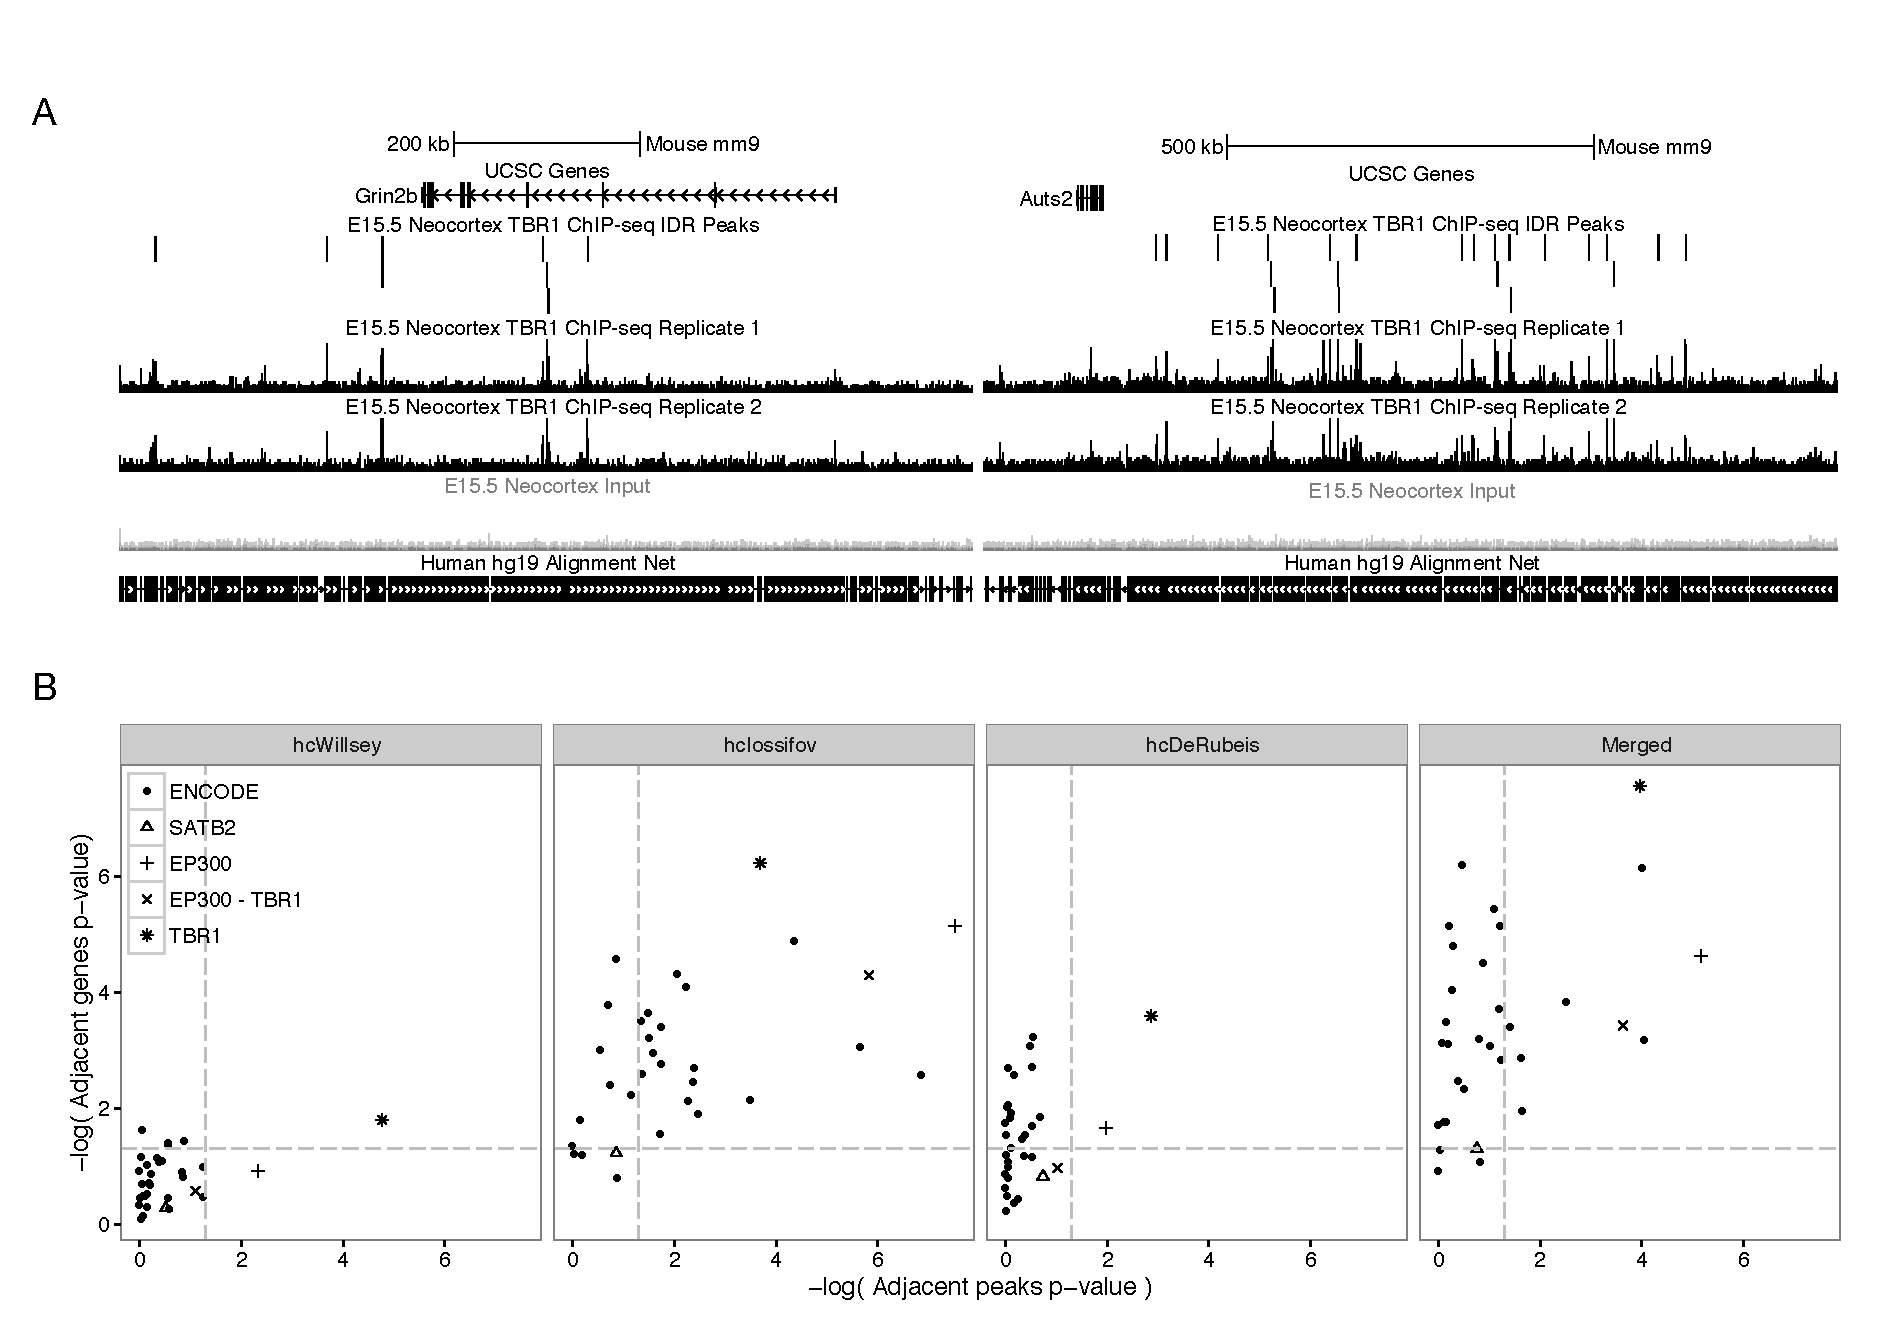
\epsfig{file=figures/autismFigure1.pdf,width=0.99\linewidth,clip=,trim=0 0 0 0} \\
\end{tabular}
\caption[TBR1 binds near high-confidence ASD genes]{
{\bf TBR1 binds near high-confidence ASD genes.}
{\bf (A)} Regulatory domains of \emph{Grin2b} with 8 adjacent TBR1 ChIP-seq peaks and \emph{Auts2} with 22 adjacent TBR1 ChIP-seq peaks.
{\bf (B)} Significance
of the number of TBR1 ChIP-seq peaks adjacent to each high-confidence
ASD gene set given the total number of peaks and size of the genomic
regions used to associate peaks with their adjacent genes (the negative
logarithm of the GREAT binomial \emph{p}-value; x-axis) compared to the
significance of the number of high-confidence ASD genes with an adjacent
TBR1 peak given the total number of genes with an adjacent TBR1 peak
(negative logarithm of the GREAT hypergeometric \emph{p}-value; y-axis).
Enrichment compared to E14.5 neocortex EP300 ChIP-seq, E15.5 neocortex
SATB2 ChIP-seq, and 28 ENCODE ChIP-seq sets including tissues at
different developmental time-points and primary cell lines. Dashed gray
lines represent \emph{p} = 0.05 significance level.
}
\label{fig:autismFig1}
\end{figure}

To test the hypothesis that ASD genes are transcriptionally regulated by
TBR1, we performed ChIP-seq for TBR1 on mouse whole cortex dissected
from embryonic day 15.5 (E15.5) embryos, a stage at which deep cortical
layers have already been generated and are completing their migration~\citep{McConnell:1991hh,Molyneaux:2007hy}, and identified 7,324 TBR1
ChIP-seq peaks (see Methods in \ref{sec:autismMethods}). These peaks significantly overlap TBR1
ChIP-seq in N2A cells ~\citep{Han:2011fs} (\emph{p}-value: 4.0E-04; see
Methods in \ref{sec:autismMethods}) and are highly enriched for the known TBR1 motif~\citep{Jolma:2013fh} (\emph{E}-value: 8.3E-101; \figref{fig:autismFigS1}; see Methods in \ref{sec:autismMethods}). In
addition, our TBR1 ChIP-seq peaks were enriched for overlapping the
active enhancer marks H3K27ac (\emph{p-}value \textless{} 1.0E-04) and
H3K4me1 (\emph{p-}value \textless{} 1.0E-04), as well as H3K9me3
(\emph{p-}value = 2.0E-03) and H3K27me3 (\emph{p-}value \textless{}
1.0E-04; see Methods in \ref{sec:autismMethods}), marks associated with repressed chromatin states,
assayed in mouse E14.5 whole brain~\citep{ENCODEProjectConsortium:2012gc};
this suggests possible roles for TBR1 as both a transcriptional
activator and repressor. When we examined \emph{Grin2b} and
\emph{Auts2}, ASD genes that are regulated by TBR1~\citep{Bedogni:2010ew, Chuang:2014bc}, we observed multiple adjacent TBR1 ChIP-seq peaks
(\figref{fig:autismFig1}A). To associate TBR1 peaks with their putative target genes, we
used the established Genomic Regions Enrichment of Annotations Tool
(GREAT)~\citep{McLean:2010iq} with default parameters (see Methods in \ref{sec:autismMethods}) and
found the majority of peaks were distal to their associated
transcription start sites (\figref{fig:autismFigS2}). We then mapped each of
the high-confidence and probable ASD genes to their mouse orthologs
(\figref{fig:autismFigS3}; see Methods in \ref{sec:autismMethods}), and used GREAT to test whether TBR1
was enriched for binding near the high-confidence ASD genes, given the
number of TBR1 peaks and the size of the genomic regions used by GREAT
to associate peaks with their adjacent genes. For each set of ASD genes,
we calculated a binomial \emph{p}-value that reflects the significance
of the number of peaks adjacent to these genes, as well as a
hypergeometric \emph{p-}value that reflects the significance of the
number of these genes with adjacent peaks~\citep{McLean:2010iq}.

TBR1 bound 27 regions adjacent to 6 of the 9 hcWillsey genes (67\%,
binomial \emph{p}-value: 1.69E-05, hypergeometric \emph{p}-value:
1.59E-02), 66 regions adjacent to 20 of 27 hcIossifov genes (74\%,
binomial \emph{p}-value: 2.03E-04, hypergeometric \emph{p}-value:
5.90E-07), and 42 regions adjacent to 12 of 17 hcDeRubeis genes (71\%,
binomial \emph{p}-value: 1.35E-03, hypergeometric \emph{p}-value:
2.55E-04; \figref{fig:autismFig1}B). In addition, when we merged the high-confidence gene
sets, we found that TBR1 bound 82 regions adjacent to 25 of the 34
high-confidence ASD genes (74\%, binomial \emph{p}-value: 1.11E-04,
hypergeometric \emph{p}-value: 2.81E-08). We previously performed
ChIP-seq in E14.5 neocortex for EP300~\citep{Wenger:2013jd}, a
transcriptional co-activator that marks active enhancers, and ChIP-seq
in E15.5 neocortex for SATB2~\citep{McKenna:2015fv}, another master
regulator of cortical development. The TBR1 high-confidence ASD gene
enrichment is stronger by either the binomial or hypergeometric test
than the enrichments for EP300 or SATB2. Furthermore, when the EP300
peaks overlapped by TBR1 are removed, the remaining EP300 peaks show no
statistical enrichment for 2 of the 3 high-confidence ASD gene lists
(\figref{fig:autismFig1}B). In addition, The ENCODE Project Consortium performed ChIP-seq
for 9 transcription factors in different subsets of 20 primary cells and
tissues from mouse~\citep{ENCODEProjectConsortium:2012gc}. This includes
brain related tissues, including E14.5 whole brain, 8-week olfactory
bulb, 8-week cerebral cortex, and 8-week cerebellum. TBR1 is more
enriched for binding adjacent to every high-confidence ASD gene set by
either the binomial or hypergeometric statistic than each of the ENCODE
ChIP-seq experiments (\figref{fig:autismFig1}B). As TBR1 is
enriched adjacent to each high-confidence gene set individually, as well
as the merged set, we used the merged set of high-confidence ASD genes
for all subsequent analyses. Together, these results suggest that the
enrichment for TBR1 peaks adjacent to high-confidence ASD genes is not
the consequence of these ASD genes being actively transcribed in the
neocortex, but a specific property of TBR1.

Giving rise to these enrichments, TBR1 binding reflects a particularly
dense pattern of regulation. In addition to using GREAT to measure the
enrichment of our TBR1 ChIP-seq peaks adjacent to a set of genes, we can
also use GREAT to measure the significance of observing a given number
of peaks next to each gene individually. Doing so, we observe as many as
10 TBR1 ChIP-seq peaks adjacent to a single high-confidence ASD gene
(\emph{Dscam}; GREAT binomial \emph{p-}value: 3.58E-04), 8 peaks
adjacent to the previously known target \emph{Grin2b} (GREAT binomial
\emph{p-}value: 7.25E-03; \figref{fig:autismFig1}A), and an average of more than 2
adjacent TBR1 ChIP-seq peaks per high-confidence ASD gene overall. In
our previous study of E14.5 mouse neocortex, we observed that
\emph{Auts2} has 29 adjacent EP300 ChIP-seq peaks~\citep{Wenger:2013jd}.
In this study, we found that \emph{Auts2} has 22 adjacent TBR1 peaks
(GREAT binomial \emph{p-}value: 1.12E-11; \figref{fig:autismFig1}A).

Gene co-expression, protein-protein interactions, and combinations of
these together with candidate genes have been used to construct gene
modules that were enriched for ASD genes. Parikshak \emph{et al}.
constructed gene networks from gene expression data collected by
RNA-seq. Their M3 module was enriched for DNA binding and
transcriptional regulation; it also included \emph{TBR1} among 996 genes
and was one of two modules significantly enriched for rare \emph{de
novo} variants from ASD probands and superficial cortical layers~\citep{Parikshak:2013di}. 662 of our TBR1 ChIP-seq peaks were enriched
for binding adjacent to genes from this module, but the 228 genes with
adjacent peaks were not significant (GREAT binomial \emph{p}-value:
5.77E-16, GREAT hypergeometric \emph{p}-value: 0.30). In contrast, Li
\emph{et al.} constructed networks from protein interaction data; they
identified a group of genes, termed module \#13, that included
\emph{TBR1} among 119 genes, which was one of two modules enriched for
ASD genes, and included genes expressed ubiquitously throughout the
brain and in the corpus callosum~\citep{Li:2014ft}. Our TBR1 ChIP-seq
peaks were not enriched for binding adjacent to genes from this module,
but the 65 genes with adjacent peaks were significant (GREAT binomial
\emph{p}-value: 0.24, GREAT hypergeometric \emph{p}-value: 1.18E-10).
Finally, Hormozdiari \emph{et al.} used a combination of co-expression,
protein-protein interactions, and genes with mutations enriched in ASD
and intellectual disability cases but not controls. Their M1 extended
network included \emph{TBR1} among 80 genes and was associated with
chromatin remodeling and the Wnt and Notch signaling pathways~\citep{Hormozdiari:2015ih}. Here, we observed no significant enrichment
(GREAT binomial \emph{p}-value: 0.35, GREAT hypergeometric
\emph{p}-value: 0.18), possibly due to the inclusion of missense
mutations or genes mutated in individuals with intellectual disability.
Together, these reflected less consistent enrichments than those for the
high-confidence ASD genes.

\subsection{High-confidence ASD genes are mis-regulated in \emph{Tbr1} KOs }

\begin{center}
\begin{longtable}
{@{}p{0.3\linewidth}p{0.3\linewidth}p{0.3\linewidth}@{}}
\caption[High-confidence ASD genes are mis-regulated in
\emph{Tbr1} knockouts]{{\bf High-confidence ASD genes are mis-regulated in
\emph{Tbr1} knockouts.}
High-confidence ASD genes are highly enriched
among genes differentially expressed in \emph{Tbr1} KOs in E14.5
neocortex from Bedogni \emph{et al}.
}
\label{tab:autismTab2} \\

\hline ~ & \textbf{ASD genes} & \textbf{w/ TBR1 ChIP-seq peak} \\ \hline 
\endfirsthead

\hline ~ & \textbf{ASD genes} & \textbf{w/ TBR1 ChIP-seq peak} \\ \hline 
\endhead

\hline
\endlastfoot

Fraction differentially expressed in \emph{Tbr1\textsuperscript{-/-}} &
15 / 33 (45\%) & 12 / 15 (80\%)\tabularnewline
Hypergeometric \emph{p}-value & 1.39E-08 & 1.68E-05\tabularnewline
\end{longtable}
\end{center}

To determine whether TBR1 binding affects the expression of putative
target genes, we first analyzed published microarray data to investigate
differences in gene expression between \emph{Tbr1}\textsuperscript{+/+}
and \emph{Tbr1}\textsuperscript{-/-} E14.5 mouse whole neocortex~\citep{Bedogni:2010ew}. Differentially expressed probes corresponded to
1,784 of 21,524 genes (8\%) assayed on the array (see Methods in \ref{sec:autismMethods}). TBR1
ChIP-seq peaks were significantly enriched adjacent to the
differentially expressed genes (658 genes, GREAT binomial
\emph{p}-value: 1.59E-29, GREAT hypergeometric \emph{p-}value:
3.54E-36). After excluding \emph{Tbr1} itself from the merged gene list,
we found that 15 of the 33 high-confidence ASD genes (45\%,
hypergeometric \emph{p}-value: 1.39E-08) showed altered expression in
\emph{Tbr1} mutant cortices at E14.5 (\tabref{tab:autismTab2}; see Methods in \ref{sec:autismMethods}). Overall,
the microarray differentially expressed genes were congruent with the
high-confidence genes that had adjacent TBR1 ChIP-seq peaks (excluding
\emph{Tbr1}): 12 of 15 differentially expressed high-confidence ASD
genes had at least one adjacent TBR1 ChIP-seq peak (80\%, hypergeometric
\emph{p}-value: 1.68E-05; \tabref{tab:autismTab2}). Together, these results suggest that
TBR1 binding influences high-confidence ASD gene expression and is
likely a direct transcriptional regulator of high-confidence ASD genes
in the developing neocortex.

TBR1 regulates the expression of genes in specific layers of the
developing cortex~\citep{Bedogni:2010ew}. Because microarray profiling
integrates signals from cells throughout the whole cortex and is not
intended to detect changes in subpopulations of cells, we examined the
spatial patterns of gene expression in \emph{Tbr1} mutant cortices using
\emph{in situ} hybridization. Here, we focused our analyses on 9
high-confidence ASD genes (not including \emph{Tbr1} itself) supported
by at least 3 studies: 7 from the intersection of the 3 high-confidence
ASD gene lists (\emph{ANK2, CHD8, DYRK1A, GRIN2B, KATNAL2, POGZ,
SCN2A}), and an additional 2 omitted by Willsey \emph{et al}.
(\emph{ADNP, ARID1B}) but supported by Iossifov \emph{et al.}, De Rubeis
\emph{et al.}, and earlier studies~\citep{ORoak:2011kf, ORoak:2012kb, Krumm:2014hd}.

\begin{figure}[htbp]
\centering
\begin{tabular}{l}
\epsfig{file=figures/autismFigure2.pdf,width=0.8\linewidth,clip=,trim=0 0 0 0} \\
\end{tabular}
\caption[TBR1 is necessary for ASD gene expression in specific
cortical lamina]{
{\bf TBR1 is necessary for ASD gene expression in specific
cortical lamina.}
Radioactive \emph{in situ} hybridization (RISH) of
high-confidence genes at E15.5 {\bf (A)} and P0 {\bf (B)} in
\emph{Tbr1}\textsuperscript{+/+} and \emph{Tbr1\textsuperscript{-/-}}
cortices reveal expression differences. RISH expression (lines in shades
of red) corresponds to normalized grain counts (see Methods in \ref{sec:autismMethods}), and
significance was determined using the 2-sided \emph{t}-test (see
Methods in \ref{sec:autismMethods}; \emph{n =} 3 to 6 sections encompassing 3 samples per
genotype). E15.5 cortical plate (red), P0 upper layers (brown), and P0
deep layers (pink). Upper layers correspond to layers 2-5 and deep
layers correspond to layer 6 (see Methods in \ref{sec:autismMethods}). Error bars represent s.d.
*\emph{p}-value \textless{} 0.05; **\emph{p}-value \textless{} 0.01;
***\emph{p-}value \textless{} 0.001.
}
\label{fig:autismFig2}
\end{figure}

\emph{Tbr1} is expressed soon after cortical neurons begin to
differentiate and is most highly expressed in early-born neurons of the
preplate, Cajal Retzius neurons, and layer 6~\citep{Bulfone:1995kl} (\figref{fig:autismFig2}). Our \emph{in situ} experiments revealed that 4 high-confidence ASD
genes that are expressed throughout the cortical plate are significantly
reduced in the brains of \emph{Tbr1}\textsuperscript{-/-} mice at E15.5:
\emph{Arid1b, Ank2}, \emph{Scn2a1}, and \emph{Grin2b} (\figref{fig:autismFig2}A and
\figref{fig:autismFigS5}A). Grain counts were performed to quantify \emph{in
situ} differences in expression (see Methods in \ref{sec:autismMethods}; \figref{fig:autismFig2}A and \figref{fig:autismFig2}B). We also
examined \emph{Tbr1} knockout mice at P0, when distinct cortical lamina
are visible. We observed \emph{Arid1b} expression, which is restricted
to layer 5, to significantly decrease in the knockout at P0 (\figref{fig:autismFig2}B,
\figref{fig:autismFigS4}, and \figref{fig:autismFigS5}B). In addition, \emph{Ank2}, which is
expressed throughout the cortex, and \emph{Scn2a1}, which is enriched in
the deep cortical layers, both showed an increase in expression
throughout the cortex in the P0 \emph{Tbr1} knockout (\figref{fig:autismFig2}B,
\figref{fig:autismFigS4}, and \figref{fig:autismFigS5}B). Three additional genes,
\emph{Adnp},~\emph{Dyrk1a}~and~\emph{Pogz}, are expressed diffusely
throughout the cortical layers of controls but specifically increase in
expression in the deep layers of P0 \emph{Tbr1} knockouts (\figref{fig:autismFig2}B, \figref{fig:autismFigS4}, and \figref{fig:autismFigS5}B). Collectively, the \emph{in situ}
hybridization analysis from these 2 time points showed that 7 of the 9
high-confidence ASD genes (excluding \emph{Tbr1}) were mis-expressed in
the \emph{Tbr1} knockouts. In addition, the two genes which are not
mis-expressed, \emph{Chd8} and \emph{Katnal2}, lacked adjacent TBR1
ChIP-seq peaks, while all of the mis-expressed genes, with the exception
of \emph{Pogz}, had one or more adjacent peaks. Thus, together with the
ChIP-seq data, these results are consistent with the role of TBR1 as a
direct transcriptional regulator of high-confidence ASD genes in the
developing neocortex.

\subsection{TBR1 binds near highly co-expressed genes}

In addition to being significantly enriched for binding adjacent to
genes differentially expressed from the \emph{Tbr1} knockout microarray
experiments, we also turned to the Allen Brain Atlas to identify
co-expressed genes. We identified human genes with mouse orthologs that
had patterns of expression correlated with \emph{TBR1} (r $\geq$ 0.8). TBR1
was highly enriched for binding adjacent to these genes with 157 peaks
adjacent to 51 of 87 genes (59\%, GREAT binomial \emph{p}-value:
5.89E-11, GREAT hypergeometric \emph{p}-value: 9.01E-10), further
supporting the role of TBR1 as an upstream regulator.

\subsection{TBR1 target genes are depleted for LoF mutations}

\begin{figure}[htbp]
\centering
\begin{tabular}{l}
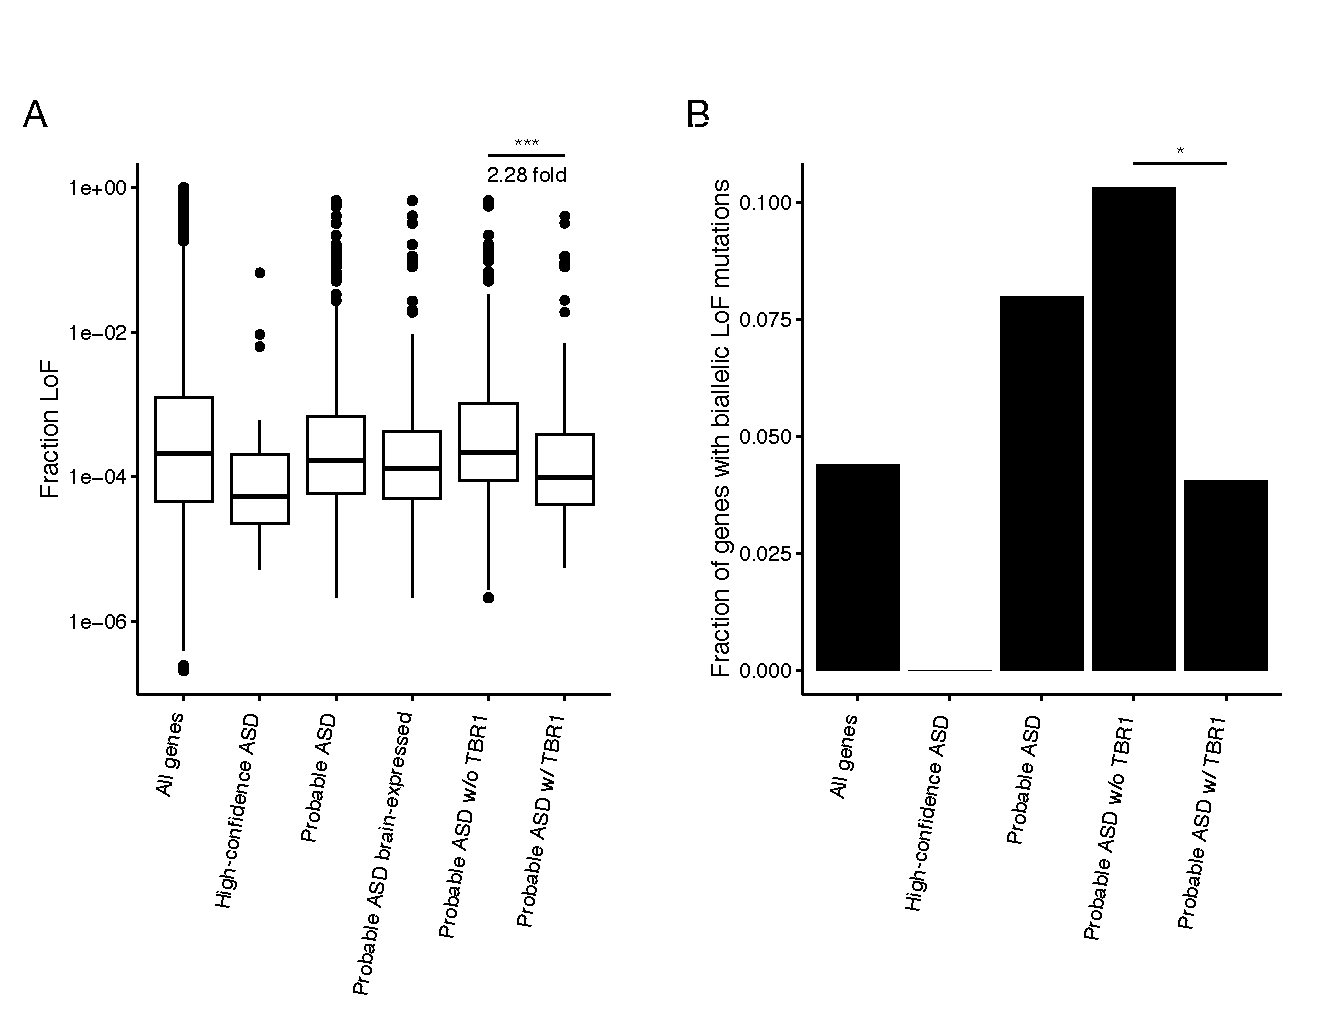
\epsfig{file=figures/autismFigure3.pdf,width=0.9\linewidth,clip=,trim=0 0 0 0} \\
\end{tabular}
\caption[Probable ASD genes that are TBR1 targets are
more depleted for ExAC LoF mutations and biallelic LoF mutations in
Icelanders]{
{\bf Probable ASD genes that are TBR1 targets are
more depleted for ExAC LoF mutations and biallelic LoF mutations in
Icelanders.}
{\bf (A)} Box-plots depicting the distributions of fraction LoF
scores for each gene from the ExAC reference population (y-axis) for
merged ASD gene lists (x-axis). Probable ASD genes with adjacent TBR1
ChIP-seq peaks in the developing cortex have lower fraction LoF scores
than those without an adjacent TBR1 peak. A pseudo-count of 1 LoF allele
for 121,412 sampled alleles, the maximum number sampled at any locus,
was included for each gene for visualization purposes. Significance was
determined using the 1-sided 2-sample Wilcoxon test. {\bf (B)} The fraction of
genes in each gene list with biallelic mutations in a study of Icelandic
individuals~\citep{Sulem:2015fi}. Significance was determined using the
1-sided Fisher's exact test. *\emph{p}-value \textless{} 0.05;
***\emph{p-}value \textless{} 0.001.
}
\label{fig:autismFig3}
\end{figure}

The heterozygous nature of \emph{de novo} LoF mutations~\citep{Iossifov:2014if}, suggests that the affected genes were haploinsufficient and that
putative ASD genes are under strong selective pressure. To test this
idea, we examined the frequency of LoF mutations in ASD genes in a large
control population from the Exome Aggregation Consortium (ExAC), which
aggregated exome sequencing data from 60,706 unrelated individuals,
excluding individuals diagnosed with severe pediatric diseases~\citep{Consortium:2015ib}. For each gene in the ExAC Browser,
we computed the proportion of mutations that were LoF (fraction LoF; by
computing the proportion of mutations that are LoF, we control for gene
length and sequence context; see Methods in \ref{sec:autismMethods}) to
assess the frequency of LoF alleles. We discovered that high-confidence
ASD genes were depleted for LoF mutations (\figref{fig:autismFig3}A). Furthermore,
\emph{TBR1} was the only high-confidence ASD gene in which no LoF
mutations were observed in the ExAC population.

As discussed above, the probable ASD genes are thought to be a
combination of true ASD genes, as well as unrelated incidental findings.
We found that the probable ASD genes were skewed toward a higher
fraction of LoF alleles in the ExAC population (\figref{fig:autismFig3}A). Previous
estimates suggested that only half of the probable ASD genes represented
true ASD risk genes~\citep{Willsey:2013bd}. We used our TBR1 ChIP-seq
results to divide the probable ASD genes with mouse orthologs into two
groups: those with and without a TBR1 ChIP-seq peak adjacent to their
ortholog (173 of 464 probable ASD genes had adjacent ChIP-seq peaks;
\tabref{tab:autismTabS1}). We then compared the probable ASD genes having
at least one adjacent TBR1 ChIP-seq peak to the remaining genes and
found that the genes having adjacent TBR1 ChIP-seq peak(s) were over
2-fold depleted for LoF mutations (2-sample Wilcoxon \emph{p}-value:
3.87E-06 and fold of medians: 2.28; \figref{fig:autismFig3}A). In addition, the genes
having at least one adjacent TBR1 ChIP-seq peak were nominally depleted
for LoF mutations compared to brain expressed genes (2-sample Wilcoxon
\emph{p}-value: 0.11 and fold of medians: 1.33), although this was a
harsh comparison due to overlap between the two sets. We observed the
same trends when using a different mutation tolerance metric, the
Residual Variation Intolerance Scores~\citep{Petrovski:2013bp} (RVIS;
\figref{fig:autismFigS6}; see Methods in \ref{sec:autismMethods}). Therefore, TBR1 binding allowed us
to identify an appealing subset of probable ASD genes that were less
tolerant to LoF alleles, as reflected by a lower fraction LoF in the
reference data set (\tabref{tab:autismTab3}).

\begin{center}
\begin{longtable}
{@{}p{0.2\linewidth}p{0.2\linewidth}p{0.2\linewidth}p{0.2\linewidth}p{0.2\linewidth}@{}}
\caption[Probable ASD genes that are neocortical transcriptional
targets of TBR1 and less tolerant to LoF alleles]{{\bf Probable ASD genes that are neocortical transcriptional
targets of TBR1 and less tolerant to LoF alleles.}
19 probable ASD genes
enriched for TBR1 ChIP-seq peaks adjacent to their mouse ortholog based
on the GREAT single-gene binomial test and fraction LoF scores less than
1.0E-3.
}
\label{tab:autismTab3} \\

\hline ~ & \textbf{LoF \textless{} 5E-05} & \textbf{LoF \textless{} 2E-04} & \textbf{LoF \textless{} 1E-03} \\ \hline 
\endfirsthead

\hline ~ & \textbf{LoF \textless{} 5E-05} & \textbf{LoF \textless{} 2E-04} & \textbf{LoF \textless{} 1E-03} \\ \hline 
\endhead

\hline
\endlastfoot

Peaks \emph{p}-value \textless{} 1E-03 & \emph{NFIA, NFIB, ZBTB18} &
\emph{CUX2, LRP6} & ~\tabularnewline
Peaks \emph{p}-value \textless{} 1E-02 & \emph{MYT1L, PBX1} &
\emph{FAM8A1, IGSF3, ZFHX3} & \emph{INSC}\tabularnewline
Peaks \emph{p}-value \textless{} 5E-02 & \emph{PPP1R15B, RELN} &
\emph{CMPK2, NIN, WNT7B} & \emph{BRCA1, CECR2, GSDMC}\tabularnewline
\end{longtable}
\end{center}

\subsection{TBR1 target genes have fewer biallelic LoF mutations}

More than a thousand non-essential genes with homozygous or compound
heterozygous LoF mutations have been identified by genomic sequencing of
2,636 individuals and genotyping of an additional 101,584 subjects in
Iceland, who were selected because they were affected by common diseases
of adulthood~\citep{Sulem:2015fi}. We investigated whether ASD genes,
particularly those regulated by TBR1, were less likely to have biallelic
LoF mutations in this population. None of the high-confidence ASD genes
had biallelic LoF mutations in the Icelandic population (\figref{fig:autismFig3}B). As
above, we split the lists of probable ASD genes with mouse orthologs
into those with and without a TBR1 ChIP-seq peak adjacent to their
ortholog (\tabref{tab:autismTabS1}). Genes with adjacent TBR1 peaks were
less likely to show biallelic LoF mutations when compared to those
without, with odds ratios of 0.37 (Fisher's exact test \emph{p-}value:
1.05E-02; \figref{fig:autismFig3}B). These results provide additional evidence that TBR1
regulates a group of ASD genes that are intolerant to LoF mutations.

\section{Discussion}

Statistical evidence has suggested that between 300 and 1,000 genes
could confer increased ASD risk~\citep{Krumm:2014hd}. Discovering
high-confidence ASD genes is a significant challenge, however, because
recurrent mutations in any given gene are uncommon~\citep{Yu:2013im}.
Recent exome sequencing studies on large cohorts composed of thousands
of individuals have revealed 35 high-confidence ASD genes with recurrent
\emph{de novo} LoF mutations. Among these is \emph{TBR1}, a master
regulator of cortical development. Our study reveals that many
high-confidence ASD genes have the shared mechanism of being direct
transcriptional targets of TBR1 in the developing neocortex. This
regulation is due to distal TBR1 binding and reflects a particularly
dense pattern of regulation, which we have previously found to identify
important genes for cortical development~\citep{Wenger:2013jd}. In
addition to showing that TBR1 regulates ASD genes, our study reveals the
regulatory sequences that are bound by TBR1, which will likely be useful
for interpreting non-coding ASD variants.

Our observations were made during cortical neurogenesis, highlighting
the developing neocortex as a brain region relevant to ASD. The increase
of high-confidence ASD gene expression in the deep layers of the
\emph{Tbr1} mutants is consistent with the role of TBR1 as a regulator
of deep layer cortical identity and calls attention to deep layer
cortical neurons, which have previously been implicated in ASD~\citep{Willsey:2013bd}. This is in contrast to the less consistent enrichments of
TBR1 peaks adjacent to genes that were part of modules enriched for ASD
genes from other studies~\citep{Parikshak:2013di, Li:2014ft, Hormozdiari:2015ih}. TBR1 has known roles in the neocortex as both
an activator (i.e. of \emph{Auts2;}~\citep{Bedogni:2010ew}) and a repressor
(i.e. of \emph{Fezf2;}~\citep{Han:2011fs, McKenna:2011ew}), which
explains the up and down-regulation of different genes in \emph{Tbr1}
mutant mice, and is consistent with the enrichments we observed for both
active and repressed chromatin marks. Given that the mutations observed
in ASD probands are presumed LoF, the fact that TBR1 acts as a repressor
may be surprising. At E15.5, however, all of the genes with observed
changes in expression were down regulated in the \emph{Tbr1} mutants,
suggesting that early corticogenesis may be a~key time point~in~ASD
pathology. In addition, the aberrant expression of these genes in the
\emph{Tbr1} mutants, up or down, may reflect the importance of their
levels of activity in the deep cortical layers. We also observed
instances of the same gene being activated and repressed by TBR1, i.e.
\emph{Ank2} and \emph{Scn2a1}, at different time points. In addition to
observing this in a previous study~\citep{McKenna:2015fv}, the fact that
we observe the same trend of activation and repression across RISH
\emph{in situ}, DIG \emph{in situ}, and RT-qPCR gives us confidence that
such temporal changes in regulation are possible, perhaps due to
different roles of TBR1 in different cell types, but understanding this
phenomenon will require further study. Finally, the changes in
expression were observed in homozygous mutant mice, whereas the LoF
mutations observed in ASD probands affect a single allele. Given the
haploinsufficient nature of \emph{TBR1}, we expect the changes to gene
expression in the heterozygous model to be more subtle, yet still
relevant to the pathology of ASD.

TBR1's role as a master regulator of cortical development has long made
it a candidate regulator of ASD genes~\citep{Bedogni:2010ew, Chuang:2015dw}; here, we measure its binding genome-wide in the developing
cortex and confirm its role in regulating other high-confidence ASD
genes for the first time. The enrichment of TBR1 ChIP-seq peaks adjacent
to high-confidence ASD genes suggests that TBR1 can be used to select a
subset of probable ASD genes that are less tolerant to LoF alleles and
could be more relevant to ASD (\tabref{tab:autismTab3}). Testing this hypothesis
required a method to compare the relative tolerance of different genes
to mutations. A previous study found that exons that were highly
expressed in the brain and contained relatively few non-synonymous
mutations were enriched for \emph{de novo} mutations found in ASD
probands~\citep{Uddin:2014dg}. This methodology, however, failed to
produce significant findings for entire genes. Recurrent \emph{de novo}
LoF mutations found in the same gene among ASD probands are thought to
identify high-confidence ASD genes due to the differing rates of
\emph{de novo} LoF mutations in affected versus unaffected siblings~\citep{Iossifov:2014if}. In addition, the pattern of LoF mutations
observed in ASD exome sequencing studies suggests that these mutations
are heterozygous~\citep{Iossifov:2014if}, and that the evidence of
selection may be visible by examining allele frequencies in a large
reference population, such as the one compiled by ExAC. We captured
these observations in the fraction LoF metric, which controls for
length, GC-bias, and other factors by measuring the rate of LoF
mutations relative to all mutations. Using this metric, we confirm our
hypothesis and show that TBR1 can be used to select an appealing subset
of probable ASD genes that are less tolerant to LoF alleles and could be
more relevant to ASD. Against the background of all probable ASD genes,
the mouse orthologs of probable ASD genes with at least one adjacent
TBR1 ChIP-seq peak are most enriched for encoding proteins located in
the synapse, the same enrichment observed by De Rubeis \emph{et al}.,
across all of the Gene Ontology~\citep{GeneOntologyConsortium:2015fz}; out
of 22 probable ASD gene orthologs annotated with synapse, 18 have at
least one adjacent TBR1 peak (Bonferroni hypergeometric \emph{p}-value:
1.38E-02; \tabref{tab:autismTabS2}). Above, we examined the enrichment of
TBR1 ChIP-seq peaks adjacent to the genes in previously discovered
autism gene modules. We can also look at the overlap of only the
probable ASD genes with at least one adjacent TBR1 ChIP-seq peak and
these different gene modules; we find this subset of genes enriched in
the networks identified by Parikshak \emph{et al.} (15 genes,
hypergeometric \emph{p}-value: 2.66E-04), Li \emph{et al.} (4 genes,
hypergeometric \emph{p}-value: 6.60E-03), and Hormozdiari \emph{et al.}
(8 genes, hypergeometric \emph{p}-value: 5.81E-08), suggesting a level
of molecular convergence. In addition, we observed that high-confidence
ASD genes are strongly depleted for LoF mutations and never have
biallelic LoF mutations in the sequenced Icelandic population~\citep{Sulem:2015fi}. \emph{TBR1} is also the only high-confidence ASD gene with no
LoF mutation in the ExAC population, providing additional evidence that
this gene is under strong selective pressure.

Protein-protein interaction networks have previously been proposed to
identify novel ASD candidate genes based on their proximity and
connectivity to high-confidence ASD genes, forming an iterative process
by which genetics and interaction networks mutually inform~\citep{Krumm:2014hd}. Based on the current study, being a target of TBR1 in the
developing cortex and having a low LoF mutation burden can be used as
signals for the prioritization of probable ASD genes for targeted
re-sequencing and study in animal models. TBR1 binding and the fraction
LoF metric allow for the reinterpretation of even high-confidence ASD
genes. \emph{KATNAL2}, a high-confidence ASD gene for which we find no
evidence of TBR1 regulation, has a fraction LoF that is almost an order
of magnitude higher than all other high-confidence ASD genes, suggesting
that the recurrent \emph{de novo} mutations in this gene reflect weak
constraint rather than essential function in ASD. A recent study showed
that LoF variants in \emph{KATNAL2} were passed from an unaffected
mother to their unaffected male child, reinforcing this point~\citep{Iossifov:2015gi}. This methodology may even be applied to genes that have
not been previously implicated in ASD. For example, \emph{CTNND2} was
recently implicated as a critical gene in autism based on studies of
female-enriched multiplex families~\citep{Turner:2015jb} but was not
found in any of the gene lists used for the current study. Its mouse
ortholog has 7 adjacent TBR1-bound regions, and a low LoF burden. Our
methodology highlights a small set of probable ASD genes with similar
properties, including well-known cortical genes such as \emph{NFIA},
\emph{NFIB,} \emph{ZBTB18}, \emph{CUX2}, and \emph{LRP6} as well as
attractive candidates such as \emph{MYT1L} and \emph{PBX1} (\tabref{tab:autismTab3}).
Together, our findings highlight a TBR1-regulated network of ASD genes
in the developing neocortex that are relatively intolerant to LoF
mutations, indicating that these genes may play critical roles in normal
cortical development.

\section{Methods}
\label{sec:autismMethods}

\subsection{Animals}

All animal work was carried out in compliance with the University of
California at Santa Cruz IACUC, Stanford University IACUC under approved
protocols \#18487 and \#21758, University of California at San Francisco
IACUC under approved protocol \#AN098262-01I, and institutional and
federal guidelines. The day of vaginal plug detection was designated as
E0.5. The day of birth was designated as P0.

\subsection{ChIP-seq}

Chromatin immunoprecipitation followed by deep sequencing (ChIP-seq) was
performed as previously described~\citep{Eckler:2014jd, McKenna:2011ew}. Cortices dissected from E15.5 embryos were fixed for 10 min with
1\% formaldehyde and neutralized with glycine. The cells were lysed and
the chromatin was sheared into \textasciitilde{}300 base pair (bp)
fragments. Immunoprecipitation reactions were performed in duplicate
using the Rabbit anti TBR1 (Abcam: ab31940, RRID: AB\_0) antibody, which
was previously validated for ChIP-qPCR~\citep{McKenna:2011ew}.
Sequencing libraries were generated from the ChIP-ed DNA and input DNA
for control using the Illumina TruSeq kit according to the
manufacturer's protocol (\tabref{tab:autismTabS3}). 20 million cells were
used for each ChIP-seq experiment. Sequencing was performed on an
Illumina HiSeq 2000 at the UCSC Genome Technology Center. Sequencing
reads were mapped to the mouse reference genome (NCBI37/mm9) using
version 0.7.12-r1039 of the BWA sampe and aln mapping algorithms (Li and
Durbin 2009) with default parameters. ChIP-seq quality was assessed
using phantompeakqualtools version 2.0
(\url{https://code.google.com/p/phantompeakqualtools/}) and all replicates
received the highest quality score (\tabref{tab:autismTabS3}) based on the
relative strand cross-correlation coefficient (RSC). Peaks were called
using MACS version 2.1.0 20140616 with a \emph{p}-value cutoff of 0.01
and merged using the Irreproducible Discovery Rate (IDR) framework~\citep{Li:2011eo} October 2010 version using a threshold of 0.01 as
previously described
(\url{https://sites.google.com/site/anshulkundaje/projects/idr}).

For computing the overlap with TBR1 ChIP-seq performed in N2A cells,
reads were last downloaded from the Sequence Read Archive (accessions:
SRR1016884 and SRR1016885) on October 19, 2015. Sequencing reads were
mapped to the mouse reference genome (NCBI37/mm9) using version
0.7.12-r1039 of the BWA samse and aln mapping algorithms~\citep{Li:2009fi} with default parameters. The number of reads overlapping our set
of TBR1 ChIP-seq peaks was compared to the number of reads overlapping
10,000 shuffles of the same peaks across the genome (excluding the UCSC
mm9 gap track).

We downloaded H3K27ac, H3K4me1, H3K27me3, and H3K9me3 histone
modifications assayed in mouse E14.5 whole brain~\citep{ENCODEProjectConsortium:2012gc}. Enrichments with TBR1 ChIP-seq peaks were computed as
has been done previously~\citep{Notwell:2015hj}: we shuffled the TBR1
ChIP-seq peaks across the genome 10,000 times (excluding the UCSC mm9
gap track). For each shuffle, we counted the number of TBR1 peaks
overlapped by each histone modification and computed an empirical
\emph{p}-value.

Motif discovery was performed using MEME-ChIP~\citep{Machanick:2011ge} version 4.10.2 on the set of IDR peaks called from both
replicates, which were centered over the peak summits from replicate 1
of the MACS ChIP-seq peak calls and trimmed/padded to 201 base pairs,
which was approximately the median peak length.

\subsection{Gene sets}

Genes with two or more \emph{de novo} LoF mutations in ASD probands
(hcWillsey, hcIossifov, and hcDeRubeis) and genes carrying a single
\emph{de novo} LoF mutation in ASD probands (pWillsey, pIossifov, and
pDeRubeis) were obtained from refs.~\citep{Willsey:2013bd, Iossifov:2014if, DeRubeis:2014cw} respectively. Genes were mapped from human
gene symbols to mouse UCSC cluster IDs using mappings from Ensembl
Biomart (Ensembl 78)~\citep{Cunningham:2015ew}, the UCSC Genome Browser~\citep{Rosenbloom:2015bg}, and the Mouse Genome Informatics (MGI)
database~\citep{Eppig:2015ib}. Ambiguous mappings were excluded, and
mappings were validated using UCSC chains~\citep{Rosenbloom:2015bg}. All
9 hcWillsey genes and 117 of 122 pWillsey genes were mapped to their
mouse orthologs; all 27 hcIossifov genes and 312 of 326 pIossifov genes
were mapped to their mouse orthologs; and 17 of 18 hcDeRubeis genes (all
but \emph{SYNGAP1}) and 249 of 257 pDeRubeis genes were mapped to their
mouse orthologs. Additional gene lists were obtained from refs.~\citep{Parikshak:2013di, Li:2014ft, Hormozdiari:2015ih} and
mapped using the same procedures. Finally, genes co-expressed with
\emph{TBR1} in microarray data from the Allen Human Brain Atlas were
downloaded and mapped to their mouse orthologs. ChIP-seq peaks were
associated with genes using the default basal regulatory domain
definition of 5 kilobases (kb) upstream and 1 kb downstream plus
extensions in both directions to the nearest gene's basal domain, up to
1 Megabase (Mb). Enrichments were computed using GREAT version 2.0.2~\citep{McLean:2010iq}.

\subsection{Transcriptome profiling}

Transcriptome profiles were last downloaded from GEO (accession:
GSE22371) on March 17, 2015. CEL files were read using the
read.celfiles() function and normalized using the robust multichip
average (RMA) algorithm from version 1.30.0 of the oligo~\citep{Carvalho:2010bc} R library with default parameters. Differentially
expressed transcripts were identified using limma version 3.22.7~\citep{Ritchie:2015fa}. Probes with a limma reported \emph{p-}values
less than 0.05 were called differentially expressed, and probes were
mapped to genes using mappings from Ensembl Biomart (Ensembl 78) ~\citep{Cunningham:2015ew}.

\subsection{Radioactive \emph{in situ} hybridization}

Subjects in this study were
\emph{Tbr1}\textsuperscript{tm1Jlr}/\emph{Tbr1}\textsuperscript{tm1Jlr}~mice
and their wild-type littermates (RRID: MGI\_3040613). Radioactive
\emph{in situ} hybridization was carried out as previously described~\citep{Frantz:1994tc}, with the following modifications: riboprobes were
transcribed from embryonic mouse neocortex cDNA, and slides were exposed
for a period of three days to three weeks before developing. Primer
pairs were designed to capture as many isoforms as possible
(\tabref{tab:autismTabS4}). Specificity of the probe to the gene of
interest was verified using BLAT~\citep{Kent:2002jd}.

\subsection{Grain counts}

Coronal (P0) and sagittal (E15.5) sections through the frontal cortex
were imaged at 40x magnification such that individual silver grains were
resolved within a single plane. At E15.5, all images were cropped at the
same dimensions to contain only the cortical plate. At P0, images fully
contained either layers 2-5 or layer 6. For all quantifications, images
were chosen with similar cell densities and background levels. Grains
were counted using the ImageJ~\citep{Schneider:2012dw} Analyze Particles
tool. All counts were normalized to background counts in regions of the
brain that were negative for expression of the gene being quantified.
For each gene at each time point and genotype, three to six sections,
encompassing three different samples, were counted.

\subsection{Exome data}

The latest version 0.3 summary data were last downloaded from the Exome
Aggregation Consortium (ExAC) Browser~\citep{Consortium:2015ib} on October 22, 2015. Variants were obtained from the 60,706
unrelated individuals reported in this database. We used variant
annotations provided in the ExAC download, which were produced by the
Ensembl Variant Effect Predictor v77. For each Ensembl Gene Identifier,
we computed the fraction of non-reference LoF alleles annotated by ExAC,
e.g. nonsense, frameshift, and splice site, normalized to the total
number of non-reference alleles, adjusting for allelic sampling
differences. The fraction LoF score \emph{f} for gene \emph{i} is the
following:

\[f_{i}\; =\; \frac{\sum_{LoF\; variants}^{\; }{\frac{alternate\; allele\; count}{total\; alleles\; sampled}}}{\sum_{all\; variants}^{\; }{\frac{alternate\; allele\; count}{total\; alleles\; sampled}}}\]

This statistic internally controls for each gene's length, GC bias, and
other confounding factors. The trends and statistics we observed were
robust to the removal of intronic and less harmful variants, as well as
using only the subset of exomes from the National Heart, Lung and Blood
Institute's (NHLBI) Exome Sequencing Project (ESP). RVIS scores computed
from ExAC release 0.3 were last downloaded on October 22, 2015
(\url{http://genic-intolerance.org/data/RVIS\_Unpublished\_ExAC\_May2015.txt}),
and genes were mapped from human gene symbols to Ensembl IDs using
mappings from Ensembl Biomart (Ensembl 78) ~\citep{Cunningham:2015ew}.

\subsection{Icelandic KO data}

The list of genes homozygous or compound heterozygous for LoF mutations
with a minor allele frequency below 2\%, the same criterion used in the
study, were downloaded from Supplementary Table 4~\citep{Sulem:2015fi}
and mapped to human Ensembl identifiers.

\subsection{Quantitative real-time PCR (qRT-PCR)}

qRT-PCR was performed using SYBR Green (Bio-Rad) and a 7900HT Fast
Real-Time PCR System (Applied Biosystems). Gene-specific primers for
high-confidence ASD genes and the \emph{Eif1a} housekeeping gene (HKG)
were designed using the Primer 3 program~\citep{Rozen:2000wg}
(\tabref{tab:autismTabS5}). The expression levels of the target genes were
normalized relative to the expression levels of \emph{Eif1a} HKG, and
then expression levels between \emph{Tbr1}-knockouts and wildtype
littermates were compared as previously described~\citep{Pfaffl:2001vs, Darbandi:2009ht}.

\subsection{Digoxigenin \emph{in situ} hybridization}

E14.5 mouse embryos were fixed in 4\% paraformaldehyde (PFA) in 1X PBS
overnight at 4$^\circ$C. The brains were transferred into 30\% sucrose and
incubated overnight at 4$^\circ$C. Following the sucrose treatment, the brains
were washed in 1X PBS for 5 min at room temperature (RT) and embedded in
Tissue Tek™ O.C.T. compound. P0 mice were perfused with 4\%
paraformaldehyde (PFA) in 1X PBS, followed by an overnight post-fix in
4\% PFA in 1X PBS at 4$^\circ$C. The brains were transferred into 30\% sucrose
and incubated at 4$^\circ$C for 48 hours. Following the sucrose treatment, 20
$\mu$m samples were sectioned using LEICA SM2000R freezing microtome. 20 $\mu$m
sections were obtained from the E14.5 embedded specimen, utilizing a
LEICA CM1900 cryostat, and collected using
Superfrost Plus microscope slides (Fisherbrand).
\emph{In situ} hybridization on frozen tissue sections and digoxigenin
RNA probe labeling were performed according to the procedures previously
described~\citep{Long:2003tj, Wallace:1999us}. Hybridized probes
were detected with an AP-conjugated anti-digoxigenin Fab fragment
antibody (1:2000, Roche) and visualized using BM purple (Roche)
substrate system. Antisense riboprobes for high-confidence ASD genes
were prepared as previously described~\citep{Cobos:2005gy, Long:2003tj} 
(\tabref{tab:autismTabS6}).

\subsection{Data access}

The ChIP-seq data from this study data have been submitted to the NCBI
Gene Expression Omnibus (GEO; \url{http://www.ncbi.nlm.nih.gov/geo/}) under
accession number GSE71384.
